% \IEEEPARstart{A}{}demo file is ....

\IEEEPARstart{T}{he} improvements in memory density and computing performance resulting from CMOS scaling are shrinking since the transistor size is approaching its physical limitation. To further improve computing capability and reduce power consumption, various emerging non-volatile memory (NVM) devices are promoted, utilizing various physical properties such as ionic migration \cite{waser2010nanoionics}, phase transition \cite{wuttig2007phase}, or spintronics \cite{6853380}. They store information in the format of two or more distinct resistance states.
Resistive random access memory (RRAM) has a metal-insulator-metal (MIM) sandwich structure, where data are represented by the resistance of a conductive filament (CF) formed in the insulator (metal-oxide layer) \cite{7448912}. The formation of a CF leads to the low resistance state (LRS) by SET operation while the rupture of CF switches to the high resistance state (HRS) by RESET operation.  
With the features of relatively high density ($\sim$ 4 F$^2$/bit), high speed ($\sim$ 5 ns), ultra-low energy ($\leq$ pJ), and large resistance ratio ($10 \sim 1000$) \cite{6361301, 2019Emerging}, RRAM is considered as an excellent NVM device to implement multiplication-and-accumulation (MAC) computation in in-memory computing (IMC) architectures \cite{7950949, 8998360, 9335229} and artificial synapse in neuromorphic hardware systems \cite{8705375, 7423754, 8340055, 9369873}.

In actual experiments, however, the resistances in HRS/LRS and the voltages for set/reset operation between cycle to cycle (C2C) and device to device (D2D) vary because of the broad fluctuations of CF in RRAM device, which introduce variation and uncertainty. 
As a result, special circuitry is required for robust write and read operation. This work focuses on robust sensing circuit design for read operation to improve read reliability and reduce read bit error rate (BER).

% %% figure of section II
% \begin{figure*}[!t]
% \centerline
% {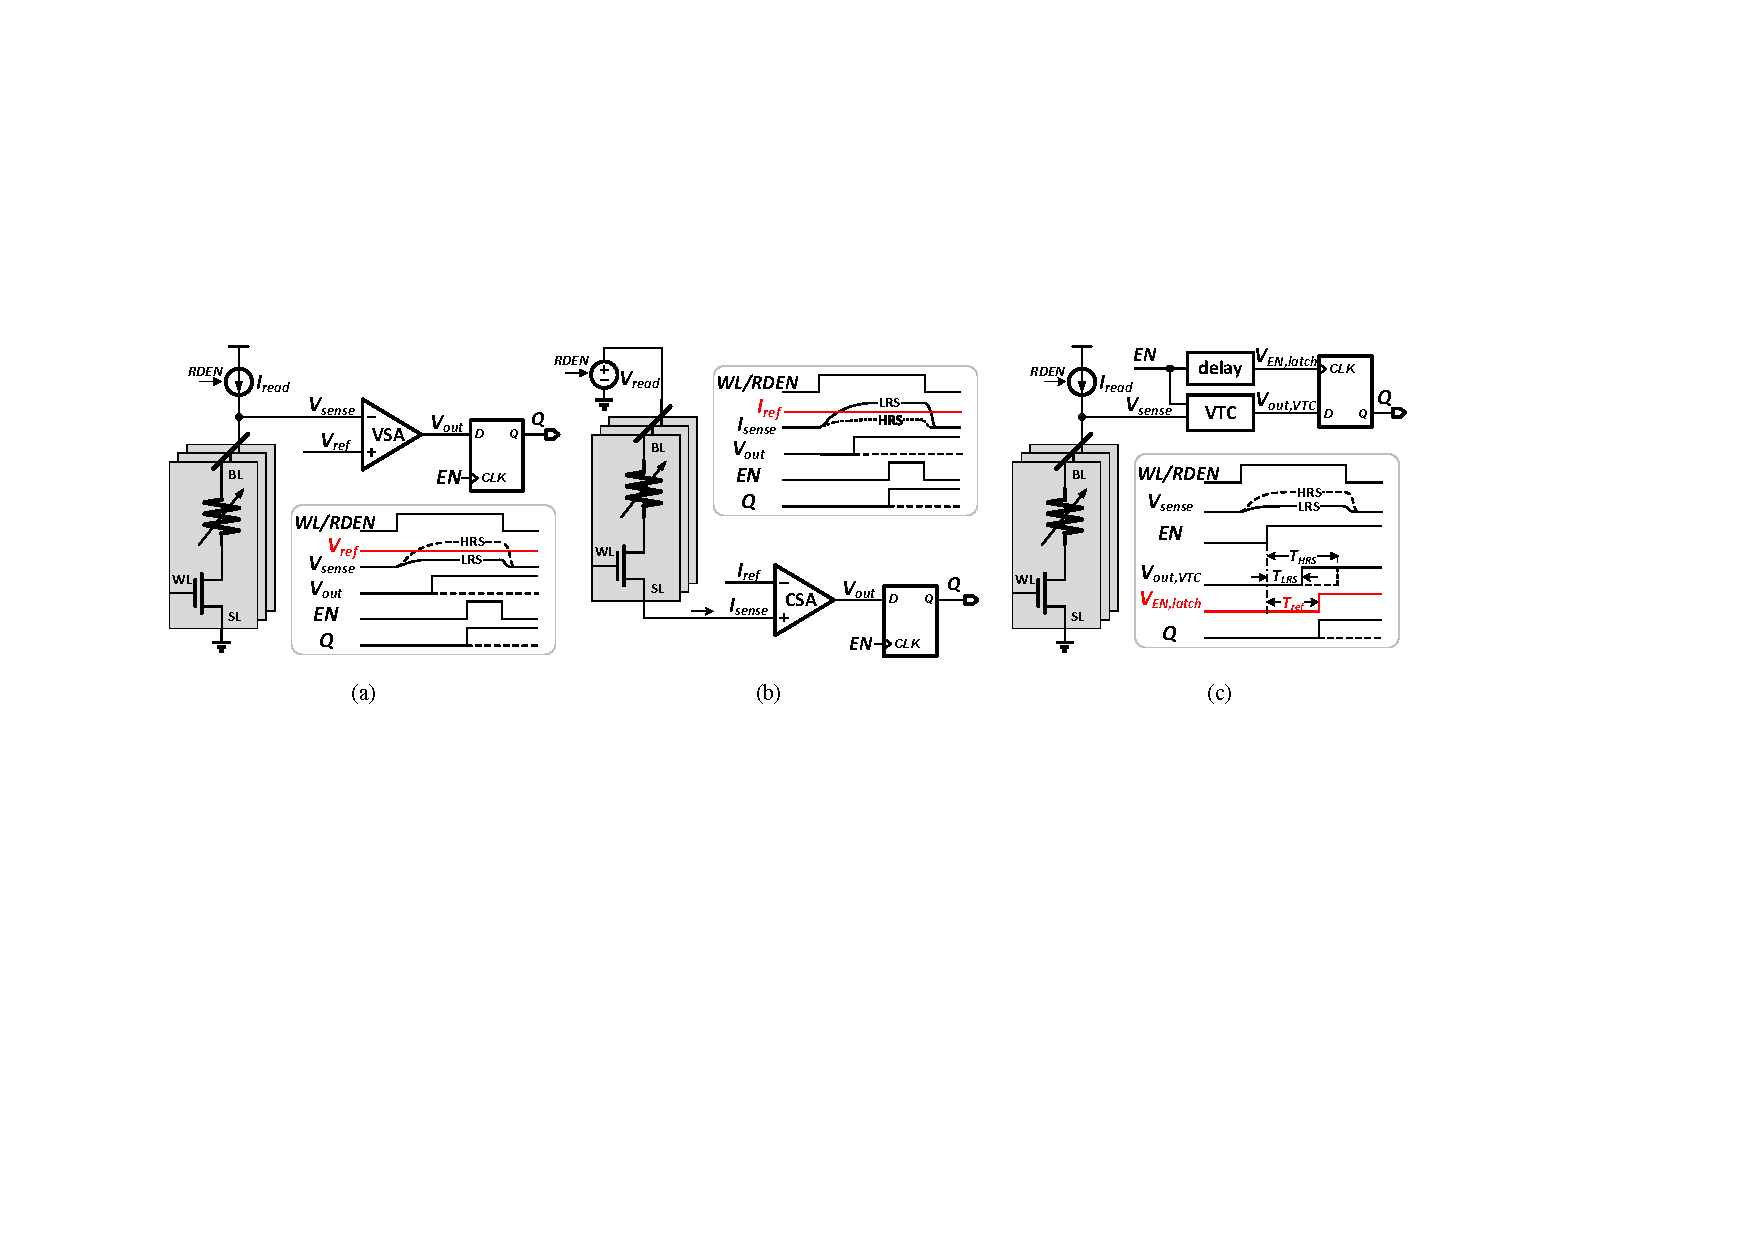
\includegraphics[width=0.95\textwidth]{fig/SA_types.pdf}}
% \caption{Conceptual circuit schematics of three different sensing schemes for NVM array. (a) Voltage mode, (b) Current mode, (c) Time mode. Assuming one specific column-wise bit line (BL) is selected.}
% \label{fig_sensing_mode}
% \end{figure*}

As a type of NVM, RRAM is suitable for applications with infrequent write operations and frequent read operations.
The energy consumption of an RRAM-based system depends largely on the readout sensing mechanism \cite{wan2020voltage}.
Therefore, the sensing performance is one of the most critical evaluations.
In general, there are three different ways to sense the data stored in RRAM by converting the data into voltage, current, and time respectively \cite{8906921}. 
% \textcolor{blue}{
The commonly used voltage mode sense amplifier (VSA) is an inverter-based latch structure \cite{yang20132mb}. However, the speed of VSA is slow, especially when bitline (BL) is too long and the resistance of RRAM in LRS is too high.
To increase the sense margin, \cite{chang201419} proposed a swing-sample-and-couple (SSC) VSA. However, the offset current affects the sensing performance. An offset-canceling (OC) current mode sense amplifier (CSA) was proposed in \cite{jain201913}. The effect of offset on the data path is eliminated by cross-sampling.
To achieve a short access time and tolerate a small read margin, \cite{lo2018reram} proposes a dynamic-trip-point-mismatch-sampling (DTPMS) CSA with small offset current and early sensing. 
On the other hand, \cite{8906921} presented a time-based sensing scheme by converting the current drawn from the bitcell to voltage pulses, which can easily distinguish the states of multi-level cell (MLC). However, the read time is too long since the number of pulses is proportional to the current’s magnitude.
% }

In this paper, we propose a novel time-based low power sensing scheme for robust reading, where the bit line (BL) voltage is converted into time delay.
It can be used for all two-terminal NVM technologies (e.g., STT-RAM, PCM, and RRAM), whose states are differentiated by the switching between a high resistance state (off-state) and a low resistance state (on-state). 
The proposed time-based sensing scheme improves the read robustness and accuracy by converting the bitcell state into time domain with the features of low power consumption and low read BER. The controller supports two different sensing modes for automatic readout. The design is scalable to multi-level sensing (MLS) that can distinguish the states of MLC. The main contributions are summarized as follows.
\begin{itemize}
  \item [1)] 
  In section \ref{sec_conv}, we describe the adopted simulation framework and clarify the particularity of the RRAM sensing methodology. The common sensing schemes based on the voltage, current, and time-domain are reviewed and compared.  
  \item [2)]
  In section \ref{sec_prop}, a time-based sensing scheme is proposed to improve the read reliability and reduce read BER. The circuit implementation and design trade-offs are analyzed. Charge-sharing-induced error compensation (CSEC) circuit is introduced to suppress charge sharing-induced error and enlarge the voltage margin of HRS and LRS, making RRAM state sensing easier and more accurate. The power gating technique enables the shaping inverter only at the sensing point to limit the short-circuit current, which is the main source of power consumption. Two operation modes of RRAM reading are supported by the timing controller circuit.
  \item [3)]
  In section \ref{sec_features}, we extend the proposed sensing scheme to MLS. This can improve sensing accuracy further by separating the sensing points for HRS and LRS. The MLS can discriminate multiple states to support MLC sensing. 
  \item [4)]
  In section \ref{sec_results}, we explore the circuit design knobs to optimize the overall performance. The simulation results are evaluated and compared with prior works. 
 %related simulation results are discussed.
  \item [5)]
  In section \ref{sec_conclusion}, we conclude this paper and summarize the benefits of the time-based sensing technique.
\end{itemize}

% The remainder of the paper is structured as follows. First, RRAM array design and the common sensing schemes are . Section \ref{sec:prop} discusses the proposed switch capacitor based PI structure and analyses the working principle. The multi-bit scaling is also discussed. Section \ref{sec:results} presents measurement results of the prototype and shows a performance comparison. Finally, the conclusions are provided in section \ref{sec:conclusion}.